\documentclass[12pt, a4paper]{article}

% --- Packages ---
\usepackage{fontspec}
\usepackage{geometry}
\usepackage{xcolor}
\usepackage{graphicx}
\usepackage{tikz}
\usepackage{booktabs}
\usepackage{array}
\usepackage{tabularx}
\usepackage{enumitem}
\usepackage{mdframed}
\usepackage{titlesec}
\usepackage{parskip}
\usepackage{hyperref}
\usepackage{fancyhdr}
\usepackage{tcolorbox}
\tcbuselibrary{skins, breakable}
\usetikzlibrary{arrows.meta, shapes.geometric, positioning, fit, backgrounds, decorations.pathreplacing}

\geometry{margin=2.5cm, top=3cm, bottom=3cm}

% --- Colours ---
\definecolor{primary}{HTML}{1A3C5E}
\definecolor{accent}{HTML}{2980B9}
\definecolor{lightblue}{HTML}{D6EAF8}
\definecolor{green}{HTML}{1E8449}
\definecolor{lightgreen}{HTML}{D5F5E3}
\definecolor{orange}{HTML}{CA6F1E}
\definecolor{lightorange}{HTML}{FDEBD0}
\definecolor{purple}{HTML}{6C3483}
\definecolor{lightpurple}{HTML}{E8DAEF}
\definecolor{grey}{HTML}{F2F3F4}
\definecolor{darkgrey}{HTML}{566573}

% --- Fonts ---
\setmainfont{Latin Modern Roman}

% --- Section styling ---
\titleformat{\section}{\Large\bfseries\color{primary}}{}{0em}{}[\color{accent}\titlerule]
\titleformat{\subsection}{\large\bfseries\color{accent}}{}{0em}{}
\titleformat{\subsubsection}{\normalsize\bfseries\color{darkgrey}}{}{0em}{}
\titlespacing{\section}{0pt}{16pt}{8pt}
\titlespacing{\subsection}{0pt}{12pt}{4pt}

% --- Header / Footer ---
\pagestyle{fancy}
\fancyhf{}
\fancyhead[L]{\small\color{darkgrey} XAI for Cross-Domain Selection Perturbative Hyper-Heuristics}
\fancyhead[R]{\small\color{darkgrey} COS790 Honours Project}
\fancyfoot[C]{\small\color{darkgrey}\thepage}
\renewcommand{\headrulewidth}{0.4pt}

% --- Callout boxes ---
\newtcolorbox{simplebox}[2][]{
  enhanced, breakable,
  colback=#2!10, colframe=#2!60,
  boxrule=0.8pt, arc=4pt,
  left=8pt, right=8pt, top=6pt, bottom=6pt,
  #1
}

\newtcolorbox{keybox}{
  enhanced, breakable,
  colback=primary!8, colframe=primary!60,
  boxrule=1pt, arc=4pt,
  left=10pt, right=10pt, top=8pt, bottom=8pt,
  fonttitle=\bfseries\color{primary},
}

% ============================================================
\begin{document}

% --- Title Page ---
\begin{titlepage}
  \centering
  \vspace*{2cm}

  {\color{primary}\rule{\linewidth}{1.5pt}}
  \vspace{0.5cm}

  {\Huge\bfseries\color{primary} How the XAI Hyper-Heuristic\\[6pt] System Works}

  \vspace{0.4cm}
  {\color{accent}\rule{0.5\linewidth}{0.8pt}}
  \vspace{0.5cm}

  {\large\color{darkgrey} A plain-English guide to the xai-sphh project\\
  from beginner to technical detail}

  \vspace{1cm}
  {\color{primary}\rule{\linewidth}{1.5pt}}

  \vspace{2cm}

  \begin{tcolorbox}[colback=lightblue, colframe=accent, arc=6pt, boxrule=1pt,
    width=0.85\linewidth, center]
    \centering
    \textbf{\large The Big Question}\\[6pt]
    \normalsize
    When a computer program is automatically solving hard problems ---
    scheduling, routing, planning --- \textbf{what is it actually learning
    to pay attention to?} And does it pay attention to the same things
    no matter which problem it is solving?
  \end{tcolorbox}

  \vfill
  {\color{darkgrey} COS790 Honours Project $\cdot$ University of Pretoria}
\end{titlepage}

% ============================================================
\tableofcontents
\newpage

% ============================================================
\section{The Big Picture (30-Second Version)}

Imagine you are trying to solve a puzzle, but you have ten different
tools available. You do not know in advance which tool is best ---
you have to try them and learn as you go.

A \textbf{hyper-heuristic} is a program that does exactly this. It sits
above a set of simple problem-solving tools (called \textbf{low-level
heuristics}) and decides at every step:

\begin{enumerate}[leftmargin=2cm]
  \item \textbf{Which tool should I use right now?}
  \item \textbf{Should I keep the result it produced, or throw it away?}
\end{enumerate}

Our project records every single one of these decisions ---
hundreds of thousands of them --- and then uses \textbf{Explainable AI}
to ask: \emph{what was the program paying attention to when it made
each decision?}

\begin{simplebox}{accent}
\textbf{Why does this matter?} Most AI decision-makers are black boxes.
You get an answer, but you do not know why. XAI opens the box and shows
you the reasoning, building trust and revealing what actually works.
\end{simplebox}

% ============================================================
\section{The Two Layers of the System}

The whole system splits into two parts that run one after the other.

\vspace{0.5cm}

\begin{center}
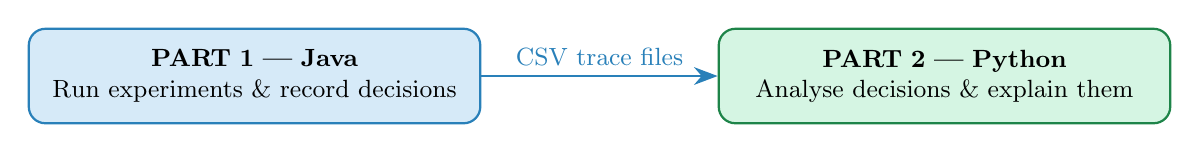
\begin{tikzpicture}[
  node distance=0.6cm,
  box/.style={rectangle, rounded corners=6pt, draw, thick,
              text width=5.5cm, align=center, minimum height=1.2cm, font=\small},
  arrow/.style={-{Stealth[length=3mm]}, thick, color=accent}
]

\node[box, fill=lightblue, draw=accent] (java)
  {\textbf{PART 1 --- Java}\\ Run experiments \& record decisions};

\node[box, fill=lightgreen, draw=green, right=3cm of java] (python)
  {\textbf{PART 2 --- Python}\\ Analyse decisions \& explain them};

\draw[arrow] (java) -- node[above, font=\small\color{darkgrey}]{CSV trace files} (python);

\end{tikzpicture}
\end{center}

\vspace{0.3cm}

\begin{itemize}
  \item \textbf{Part 1 (Java)} runs a hyper-heuristic on real benchmark problems
        and writes a detailed log of every decision made --- which tool was used,
        what the result was, and whether it was accepted.
  \item \textbf{Part 2 (Python)} reads those logs, trains an AI model to replicate
        the decision pattern, and then explains the AI model using SHAP and LIME.
\end{itemize}

% ============================================================
\section{The Problem Domains --- What Are We Actually Solving?}

The system does not run on made-up data. It runs on \textbf{six real-world
benchmark problems} from the CHeSC 2011 international competition. These are
standard test problems used by researchers worldwide.

\textbf{The data for all six problems is already bundled inside the
HyFlex jar files} (the library files in \texttt{lib/hyflex/}). You do
not import external datasets --- the instances are pre-loaded.

\vspace{0.4cm}
\begin{center}
\begin{tabularx}{\linewidth}{>{\bfseries}p{3.8cm} X p{4.5cm}}
\toprule
\textbf{Domain} & \textbf{What problem is being solved?} & \textbf{What does the score measure?} \\
\midrule
SAT
  & Find variable assignments (true/false) that satisfy a Boolean formula with thousands of clauses.
  & Number of unsatisfied clauses. \textit{Goal: reach 0.} \\[6pt]
Bin Packing
  & Pack items of varying sizes into the fewest possible bins.
  & Number of bins used. \textit{Goal: minimise.} \\[6pt]
Flow Shop
  & Schedule a set of jobs across multiple machines to finish as quickly as possible.
  & Total time to finish all jobs (makespan). \textit{Goal: minimise.} \\[6pt]
TSP (Travelling Salesman)
  & Find the shortest route that visits every city exactly once and returns home.
  & Total route distance. \textit{Goal: minimise.} \\[6pt]
VRP (Vehicle Routing)
  & Route a fleet of vehicles to serve all customers within capacity and time limits.
  & Total travel distance. \textit{Goal: minimise.} \\[6pt]
Personnel Scheduling
  & Assign staff to shifts satisfying skills, availability, and fairness rules.
  & Penalty points for broken rules. \textit{Goal: reach 0.} \\
\bottomrule
\end{tabularx}
\end{center}

\vspace{0.4cm}
Each domain has \textbf{10 pre-loaded instances} (indexed 0--9), ranging from
easy to very hard. You select which one to use in the config file using the
\texttt{instanceIndex} field.

\begin{simplebox}{orange}
\textbf{Key insight:} The hyper-heuristic \emph{never sees the actual
problem data} --- no cities, no jobs, no clauses. All it ever receives is
a single number: the objective score. This is what makes it a
\emph{cross-domain} solver. The exact same algorithm works on all six
problems without any changes.
\end{simplebox}

% ============================================================
\section{How the Hyper-Heuristic Works (High Level)}

Think of the hyper-heuristic as a student sitting an exam with a toolbox.

\begin{center}
\begin{tikzpicture}[
  node distance=0.5cm and 1.2cm,
  step/.style={rectangle, rounded corners=5pt, draw=accent, thick,
               fill=lightblue, text width=3.5cm, align=center,
               font=\small, minimum height=1.0cm},
  arrow/.style={-{Stealth[length=3mm]}, thick, color=accent}
]

\node[step] (s1) {1. Look at the\\current situation};
\node[step, right=1.5cm of s1] (s2) {2. Pick a tool\\to apply};
\node[step, right=1.5cm of s2] (s3) {3. Apply the tool\\get a new solution};
\node[step, below=1.2cm of s3] (s4) {4. Is this new\\solution better?};
\node[step, left=1.5cm of s4] (s5) {5. Keep it or\\throw it away};
\node[step, left=1.5cm of s5] (s6) {6. Learn from\\the outcome};

\draw[arrow] (s1) -- (s2);
\draw[arrow] (s2) -- (s3);
\draw[arrow] (s3) -- (s4);
\draw[arrow] (s4) -- (s5);
\draw[arrow] (s5) -- (s6);
\draw[arrow] (s6.west) -- ++(-0.5,0) -- ++(0,1.8) -- (s1.west);

\end{tikzpicture}
\end{center}

This loop runs \textbf{100,000 times} per experiment. Each pass is called an
\textbf{iteration}. At every iteration, both the selection decision (step 2)
and the acceptance decision (step 5) are recorded in the trace file.

% ============================================================
\section{Selection Strategies --- Picking the Right Tool}

There are two ways the hyper-heuristic decides which low-level heuristic to
apply next.

\subsection{Simple Random (SR) --- The Baseline}
Picks a tool completely at random. No memory, no learning. This is the
\textbf{baseline} --- we use it to compare against smarter strategies.

\subsection{Choice Function (CF) --- The Learner}
Keeps a score for every tool based on three things:

\begin{center}
\begin{tabularx}{\linewidth}{>{\bfseries}p{1cm} >{\bfseries}p{4cm} X}
\toprule
Term & Name & What it measures \\
\midrule
f1 & Individual performance & How well has this tool done on its own in the past? \\[4pt]
f2 & Pair performance & How well does this tool do \emph{after} the tool used last time? \\[4pt]
f3 & Time since last used & How long ago was this tool used? (promotes variety) \\
\bottomrule
\end{tabularx}
\end{center}

The final score is: $\text{CF}(h) = \varphi \cdot f1 + \varphi \cdot f2 + (1-\varphi) \cdot f3$

The weight $\varphi$ adapts automatically --- it jumps up when the search is
improving and slowly decays when it is not, so the system shifts between
exploiting good tools and exploring idle ones.

% ============================================================
\section{Acceptance Strategies --- Keeping or Discarding Results}

After applying a tool, the system must decide: \emph{do we keep this new
solution or stick with the old one?}

\vspace{0.3cm}
\begin{center}
\begin{tabularx}{\linewidth}{>{\bfseries}p{3.8cm} X}
\toprule
\textbf{Strategy} & \textbf{Rule} \\
\midrule
Late Acceptance (LA)
  & Accept if the new solution is at least as good as the solution from $L$ steps ago.
    Allows temporary worsening to escape local optima. \\[6pt]
AILTA
  & Adaptive version of LA. The threshold decays over time, becoming stricter as
    the budget runs out. \\[6pt]
Simulated Annealing (SA)
  & Sometimes accepts worse solutions based on probability. The chance of accepting
    bad solutions decreases over time, like metal cooling. \\[6pt]
Improving or Equal
  & Only keep if the new solution is at least as good. Simple and strict. \\[6pt]
Naive
  & Always keep. Used only for debugging. \\
\bottomrule
\end{tabularx}
\end{center}

% ============================================================
\section{Single-Point vs Multi-Point Search}

The system supports two fundamentally different search modes.

\vspace{0.3cm}
\begin{center}
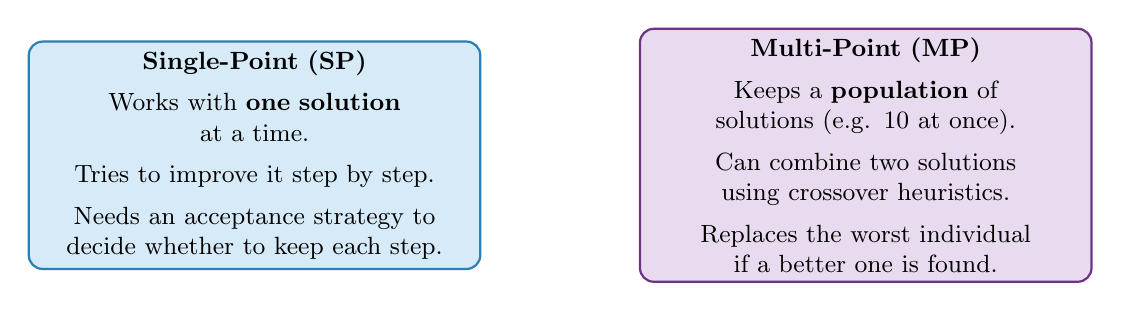
\begin{tikzpicture}[
  box/.style={rectangle, rounded corners=5pt, draw, thick,
              text width=5.5cm, align=center, font=\small,
              minimum height=2.8cm},
]
\node[box, fill=lightblue, draw=accent] (sp) {
  \textbf{Single-Point (SP)}\\[4pt]
  Works with \textbf{one solution}\\
  at a time.\\[4pt]
  Tries to improve it step by step.\\[4pt]
  Needs an acceptance strategy to\\
  decide whether to keep each step.
};

\node[box, fill=lightpurple, draw=purple, right=2cm of sp] (mp) {
  \textbf{Multi-Point (MP)}\\[4pt]
  Keeps a \textbf{population} of\\
  solutions (e.g. 10 at once).\\[4pt]
  Can combine two solutions\\
  using crossover heuristics.\\[4pt]
  Replaces the worst individual\\
  if a better one is found.
};
\end{tikzpicture}
\end{center}

\vspace{0.3cm}
For multi-point search, the replacement rule acts as acceptance --- there is no
separate acceptance strategy. An elitism guard ensures the best solution in the
population is never overwritten.

% ============================================================
\section{What Gets Recorded --- The Trace File}

Every single iteration is written to a CSV file called a \textbf{trace}.
Each row captures a complete snapshot of one decision:

\vspace{0.3cm}
\begin{center}
\begin{tabularx}{\linewidth}{>{\ttfamily\small}p{4.5cm} X}
\toprule
\textbf{Column} & \textbf{What it means} \\
\midrule
run\_id & Unique ID for this experiment run \\
iteration & Which step number this is (0 to 99,999) \\
heuristic\_id & Which low-level tool was selected \\
heuristic\_class & What type of tool: MUTATION, LOCAL\_SEARCH, etc. \\
objective\_before & Score before the tool was applied \\
objective\_after & Score after the tool was applied \\
delta & The change in score (negative = improvement) \\
accepted & Was this result kept? (true/false) \\
best\_so\_far & Best score seen at any point in the run \\
feat\_progress & How far through the budget we are (0.0 to 1.0) \\
feat\_iters\_since\_accept & How many steps since we last kept a solution \\
feat\_improve\_rate\_50 & Fraction of the last 50 steps that improved \\
feat\_pop\_diversity & How spread out the population is (MP only) \\
\ldots & (16 features total) \\
\bottomrule
\end{tabularx}
\end{center}

\vspace{0.4cm}
A single 100,000-iteration run produces a trace file of approximately 20--42 MB.
The current baseline dataset has \textbf{400,000 rows} (4 technique runs combined).

% ============================================================
\section{The Python Pipeline --- From Data to Explanation}

Once the Java side has produced trace files, the Python pipeline processes them
in six sequential stages.

\vspace{0.4cm}
\begin{center}
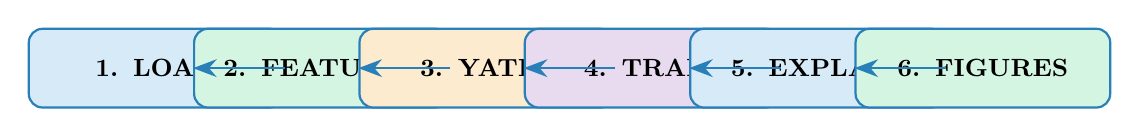
\begin{tikzpicture}[
  node distance=0.4cm,
  stage/.style={rectangle, rounded corners=5pt, draw=accent, thick,
                fill=lightblue, text width=3cm, align=center,
                font=\small\bfseries, minimum height=1cm},
  desc/.style={rectangle, align=left, text width=5.5cm, font=\small},
  arrow/.style={-{Stealth[length=3mm]}, thick, color=accent}
]

\foreach \i/\name/\col in {
  1/LOAD/lightblue,
  2/FEATURES/lightgreen,
  3/YATES/lightorange,
  4/TRAIN/lightpurple,
  5/EXPLAIN/lightblue,
  6/FIGURES/lightgreen}
{
  \node[stage, fill=\col] (s\i) at ({(\i-1)*2.1},0) {\i. \name};
}

\draw[arrow] (s1) -- (s2);
\draw[arrow] (s2) -- (s3);
\draw[arrow] (s3) -- (s4);
\draw[arrow] (s4) -- (s5);
\draw[arrow] (s5) -- (s6);

\end{tikzpicture}
\end{center}

\vspace{0.4cm}

\begin{description}[leftmargin=0cm, style=nextline]

\item[\textbf{Stage 1 --- Load}]
  Reads all CSV trace files, checks they match the schema (all 19 required columns
  present, correct data types), and saves everything into a single efficient Parquet
  file. \textit{Input: CSV files. Output: traces.parquet.}

\item[\textbf{Stage 2 --- Features}]
  Selects the 16 \texttt{feat\_*} columns as inputs to the model (X) and the
  \texttt{accepted} column as what the model must predict (y). Missing population
  features for single-point runs are filled with $-1$ (a sentinel meaning
  ``not applicable''). \textit{Output: X.parquet, y.parquet.}

\item[\textbf{Stage 3 --- Yates Measures}]
  Computes three statistical measures adapted from Yates et al.: (1) log returns
  per heuristic --- which tools give the best improvements on average; (2) percentile
  ranks of objective values; (3) footrule distance --- how much the ranking of tools
  changes between early and late search.

\item[\textbf{Stage 4 --- Train}]
  Trains a \textbf{Gradient Boosting} classifier on the 400,000 rows. The model
  learns to predict, given the state features, whether the hyper-heuristic will
  accept or reject. Performance is measured with 5-fold cross-validation.

\item[\textbf{Stage 5 --- Explain}]
  Applies SHAP and LIME to explain the surrogate model. SHAP gives a global
  picture (which features matter most across all decisions). LIME gives a local
  picture (why was this specific decision made?).

\item[\textbf{Stage 6 --- Figures}]
  Produces publication-ready PDF figures: the convergence curve (best score over
  time) and the SHAP importance bar chart.

\end{description}

% ============================================================
\section{The Explainability Layer --- SHAP and LIME}

\subsection{SHAP --- Global Explanation}

SHAP (SHapley Additive exPlanations) answers: \textbf{``which features
matter most, on average, across all 400,000 decisions?''}

It assigns each feature a score measuring how much it contributes to the
prediction. A high SHAP value means the feature strongly influences whether
the hyper-heuristic accepts or rejects.

\vspace{0.3cm}
\begin{center}
\begin{tabularx}{\linewidth}{>{\ttfamily}p{4.8cm} r X}
\toprule
\textbf{Feature} & \textbf{Mean |SHAP|} & \textbf{What it means} \\
\midrule
feat\_pop\_target\_rank   & 1.26 & Where the target sits in the population \\
feat\_pop\_diversity      & 0.99 & How spread out the population is \\
feat\_improve\_rate\_50   & 0.75 & Recent improvement frequency \\
feat\_iters\_since\_accept & 0.73 & How long since the last accepted move \\
feat\_progress            & 0.47 & How far through the budget we are \\
feat\_mean\_logret\_50    & 0.45 & Average quality of recent moves \\
feat\_iters\_since\_improve & 0.45 & How long since best score improved \\
\bottomrule
\end{tabularx}
\end{center}

\vspace{0.3cm}
\begin{simplebox}{green}
\textbf{What this tells us:} The hyper-heuristic pays most attention to
\emph{where it is in the population}, \emph{how diverse the population is},
and \emph{how recently it made progress}. It is responding to search momentum
and population structure --- not to anything problem-specific.
\end{simplebox}

\subsection{LIME --- Local Explanation}

LIME (Local Interpretable Model-agnostic Explanations) answers:
\textbf{``why was this specific decision made at iteration 50,000?''}

It creates a small perturbed dataset around a single decision and fits a simple
linear model to explain just that one prediction. Useful for auditing individual
decisions that seem surprising.

% ============================================================
\section{The Surrogate Model --- How Faithful Is It?}

Before trusting the SHAP and LIME explanations, we need to know whether the
surrogate model actually represents the real hyper-heuristic behaviour well.

\vspace{0.3cm}
\begin{center}
\begin{tabularx}{0.85\linewidth}{X r r}
\toprule
\textbf{Metric} & \textbf{Surrogate} & \textbf{Trivial baseline} \\
\midrule
Accuracy (fraction correct) & \textbf{88.5\%} & 57.5\% \\
ROC-AUC (ranking quality) & \textbf{95.3\%} & 50.0\% \\
F1 Score (balanced accuracy) & \textbf{90.5\%} & --- \\
\bottomrule
\end{tabularx}
\end{center}

\vspace{0.3cm}
The trivial baseline just always predicts the most common class. Our surrogate
is 31 percentage points better than that --- it has genuinely learned the
acceptance policy. The SHAP and LIME explanations are therefore valid
descriptions of how the hyper-heuristic actually behaves.

% ============================================================
\section{How Datasets Feed Into the System}

\begin{simplebox}{orange}
\textbf{Short answer:} You do not import your own datasets. The benchmark
problem instances are already bundled inside the HyFlex jar files. You
control which instance to run using a single number in the config file.
\end{simplebox}

\subsection{The instanceIndex Field}

Each of the six problem domains has 10 pre-loaded instances (0--9), ranging
from small and easy to large and hard. You select one using \texttt{instanceIndex}
in the YAML config:

\begin{tcolorbox}[colback=grey, colframe=darkgrey, arc=4pt, boxrule=0.6pt,
  fontupper=\ttfamily\small]
techniqueName: SP-CF-LA\\
domain: SAT\\
instanceIndex: 3\ \ \ \ \# pick instance 3 out of 10\\
seed: 42\\
budgetType: iterations\\
budgetValue: 100000\\
outputDirectory: data/raw/traces
\end{tcolorbox}

\subsection{Running the Full Experimental Matrix}

For a complete study you would run every combination of technique, domain,
instance and seed. A typical matrix:

\vspace{0.2cm}
\begin{center}
\begin{tabular}{lrl}
\toprule
\textbf{Dimension} & \textbf{Count} & \textbf{Values} \\
\midrule
Techniques & 4 & SP-SR-LA, SP-CF-LA, SP-CF-AILTA, MP-CF \\
Domains    & 6 & SAT, BinPacking, FlowShop, TSP, VRP, PS \\
Instances  & 10 & 0 through 9 \\
Seeds      & 5  & 42, 123, 456, 789, 1000 \\
\midrule
\textbf{Total runs} & \textbf{1,200} & \\
\bottomrule
\end{tabular}
\end{center}

\vspace{0.3cm}
All 1,200 trace files drop into \texttt{data/raw/traces/}. The Python pipeline
automatically picks up every CSV in that folder and combines them for analysis.

% ============================================================
\section{The Entire System in One Diagram}

\begin{center}
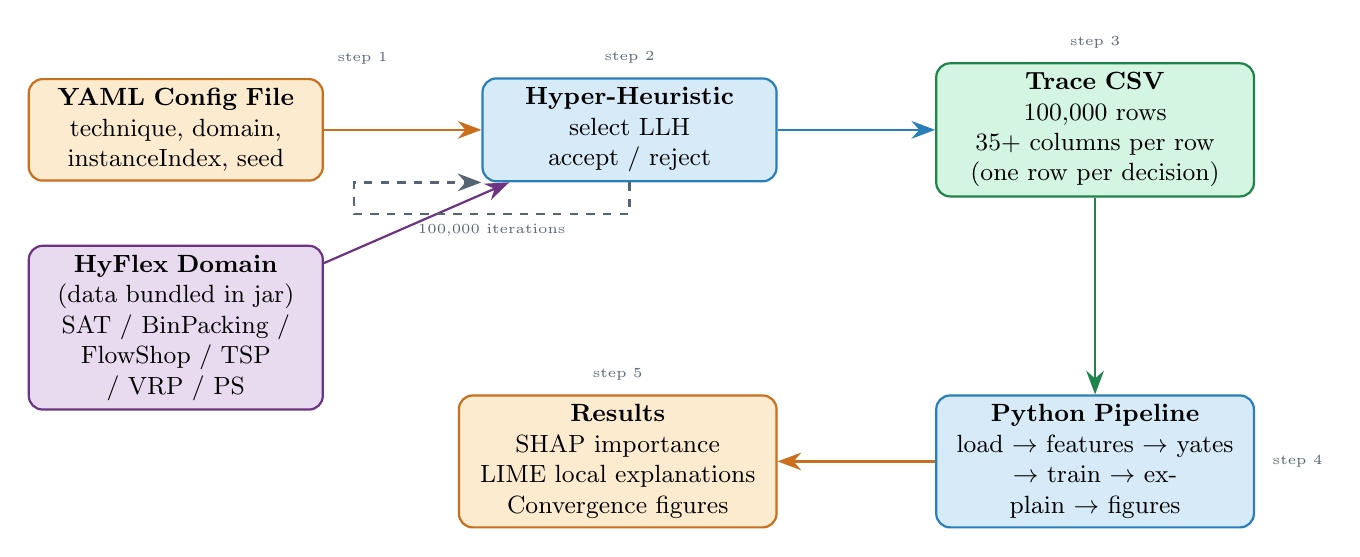
\begin{tikzpicture}[
  node distance=0.5cm and 1cm,
  box/.style={rectangle, rounded corners=5pt, draw, thick,
              align=center, font=\small, minimum height=0.9cm},
  arrow/.style={-{Stealth[length=3mm]}, thick},
  group/.style={rectangle, rounded corners=8pt, draw, dashed, thick}
]

% --- Config ---
\node[box, fill=lightorange, draw=orange, text width=3.5cm] (config)
  {\textbf{YAML Config File}\\ technique, domain,\\ instanceIndex, seed};

% --- Domain ---
\node[box, fill=lightpurple, draw=purple, text width=3.5cm, below=0.8cm of config] (domain)
  {\textbf{HyFlex Domain}\\ (data bundled in jar)\\ SAT / BinPacking /\\ FlowShop / TSP / VRP / PS};

% --- HH ---
\node[box, fill=lightblue, draw=accent, text width=3.5cm, right=2cm of config] (hh)
  {\textbf{Hyper-Heuristic}\\ select LLH\\ accept / reject};

% --- Trace ---
\node[box, fill=lightgreen, draw=green, text width=3.8cm, right=2cm of hh] (trace)
  {\textbf{Trace CSV}\\ 100,000 rows\\ 35+ columns per row\\ (one row per decision)};

% --- Python pipeline ---
\node[box, fill=lightblue, draw=accent, text width=3.8cm, below=2.5cm of trace] (pipeline)
  {\textbf{Python Pipeline}\\ load $\to$ features $\to$ yates\\ $\to$ train $\to$ explain $\to$ figures};

% --- Results ---
\node[box, fill=lightorange, draw=orange, text width=3.8cm, left=2cm of pipeline] (results)
  {\textbf{Results}\\ SHAP importance\\ LIME local explanations\\ Convergence figures};

% Arrows
\draw[arrow, color=orange] (config) -- (hh);
\draw[arrow, color=purple] (domain) -- (hh);
\draw[arrow, color=accent] (hh) -- (trace);
\draw[arrow, color=green] (trace) -- (pipeline);
\draw[arrow, color=orange] (pipeline) -- (results);

% Loop arrow
\draw[arrow, color=darkgrey, dashed]
  (hh.south) -- ++(0,-0.4) -- ++(-3.5,0)
  node[midway, below, font=\tiny\color{darkgrey}]{100,000 iterations}
  -- ++(0,0.4) -- (hh.south west);

% Labels
\node[font=\tiny\color{darkgrey}, above right=0.05cm and 0.05cm of config] {step 1};
\node[font=\tiny\color{darkgrey}, above=0.05cm of hh] {step 2};
\node[font=\tiny\color{darkgrey}, above=0.05cm of trace] {step 3};
\node[font=\tiny\color{darkgrey}, right=0.1cm of pipeline] {step 4};
\node[font=\tiny\color{darkgrey}, above=0.05cm of results] {step 5};

\end{tikzpicture}
\end{center}

% ============================================================
\section{Summary}

\begin{keybox}
\begin{enumerate}[leftmargin=0.5cm, itemsep=6pt]
  \item \textbf{The system solves real benchmark problems} from six domains
        (SAT, BinPacking, FlowShop, TSP, VRP, PersonnelScheduling) using a
        hyper-heuristic that selects and applies low-level tools automatically.

  \item \textbf{The problem data is pre-bundled.} You select which instance to
        run using \texttt{instanceIndex: 0--9} in the config file.

  \item \textbf{The hyper-heuristic is blind to the problem.} It only ever sees
        an objective score --- never cities, clauses, jobs, or routes. This is
        what makes it cross-domain.

  \item \textbf{Every decision is recorded.} A 100,000-iteration run produces a
        trace file with 100,000 rows and 35+ columns.

  \item \textbf{A surrogate AI model learns the decision pattern} (88.5\%
        accuracy) from the recorded traces.

  \item \textbf{SHAP reveals what the system pays attention to globally.}
        Population structure, search stagnation, and recent improvement rate
        dominate acceptance decisions --- not the problem type.

  \item \textbf{LIME explains individual decisions locally.} You can audit any
        specific iteration and see exactly what pushed the decision towards
        acceptance or rejection.
\end{enumerate}
\end{keybox}

\vfill
{\small\color{darkgrey}
Generated from the xai-sphh project source code. All metrics reflect the
4-technique baseline experiment (SP-SR-LA, SP-CF-LA, SP-CF-AILTA, MP-CF) run
on SAT instance 0, 100,000 iterations each.}

\end{document}
